\documentclass{CPSReport}

\setminted[python3]{breaklines, framesep=2mm, fontsize=\footnotesize, numbersep=5pt}
\usemintedstyle{friendly}

%----------------------------------------------------------------------------------------
%	AUTHOR / TITLE INFORMATION
%----------------------------------------------------------------------------------------
\title{Assignment IV: Linear Regression Models} % The article title

\author{
	\coursetitle{Introduction to Machine Learning Lab (190.013), SS2023}
	\authorstyle{Björn Ellensohn\textsuperscript{1}} % Authors
	\newline\newline % Space before institutions
	\textsuperscript{1}\textit{m01435615}, \textit{bjoern.ellensohn@stud.unileoben.ac.at}, \institution{Montanuniversität Leoben, Austria}\\ % Institution 1
	\submissiondate{\today} % Add a date here
}

%----------------------------------------------------------------------------------------
%	DOCUMENT
%----------------------------------------------------------------------------------------

\begin{document}

\maketitle % Print the title

\thispagestyle{firstpage} % Apply the page style for the first page (no headers and footers)

%----------------------------------------------------------------------------------------
%	ABSTRACT
%----------------------------------------------------------------------------------------

\lettrineabstract{This document guides through the process of solving Assignment 3.}

\section{Introduction}
The 4th assignment's task was to implement linear regression models on a provided 'diabetes' dataset.
the linear regression models had to be implemented from scratch using only numpy and pandas. the models to create where:
\begin{itemize}
    \item Least Squares Regression
    \item Ridge Regression
    \item Lasso Regression
\end{itemize}

The laste one was a bonus point task.
I will walk through the code in 4 Sections.

\section{Part I - Abstract Class}
\subsection{Preparation}
Alongside the 'diabetes.csv' dataset there was also an unfinished Jupyter Notebook provided, which gave an outline on how to solve this task. At the begin, there is an abstract class \mintinline{python}{Predictor}, that should act as a template for the child classes, implementing the actual regression models. However, I decided to extend the metaclass to include the methods that where the same for all child classe. So I only had to write them once. In my oppinion, this is better for the code's structure and enhances readability.

\subsection{Defining the Abstract Class}
The class \mintinline{python}{Predictor} is created that provides the basic outline for the main classes of this exercise. The following functions are inlcuded:
\begin{itemize}
    \item Reading the csv
    \item Loading and splitting the data into training and test sets
    \item Normalizing the data
\end{itemize}

So the dateset is loaded and will be pre-processed accordingly on initiation of the class. The needed data and paramters are stored as atributes.

To mention here are the data loading and pre processing methods. For loading the file, pandas does a good already. The pre-processing was trickier to implement. Datasets tend to have several flaws. Amongst them are outliers and missing values.
Missing data can be found with the pandas DataFrame functions \mintinline{python}{isnan} and \mintinline{python}{isnull}.
The outliers of the dataset where caught by boxplotting every column. In this case, the "1.5 x IQR rule" came to shine, as this allows to automate the process of finding the outliers for each of the columns.
The last method is the \mintinline{python}{train_test_split()} method. Here I want to split the dataset into features and targets, as well as dividing the whole dataset into a test set and a train set. This is especially useful for having a refernce for evaluating the performance later.

\section{Part II - Least Squares Regression}
In the second part of this exercise, a class \mintinline{python}{LinearRegression(Predictor)} was created to provide the actual implmentation of the linear regression.

A formula for Least Squares Regression looks like this:
\mintinline{python}{Y = b0 + b1*X1 + b2*X2 + ... + bn*Xn}, where Y is the response variable, b0 is the y-intercept, bi is the coefficient for predictor variable Xi, and Xi is the ith predictor variable.

For evaluation, the predicted data was compared to the test set, so the Mean Squared Error was measured, as well as the R-Squared.

The results are as follows. For comparison, also the unprocessed dataset was evaluated. We can already see, how bad the unprocessed set performs.

\begin{figure}[ht]
    \begin{center}
        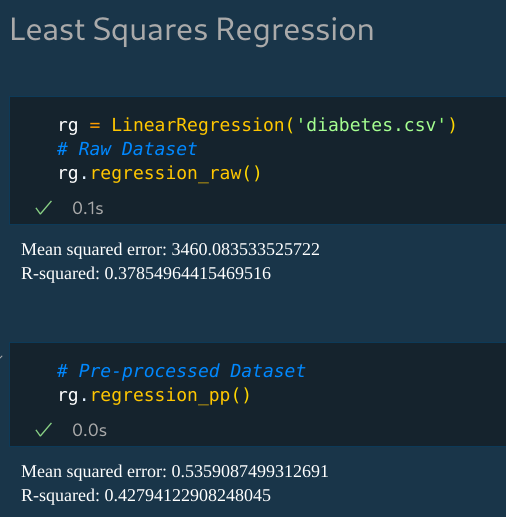
\includegraphics[width=1\linewidth]{pics/Result_Least_Squares.png}
    \end{center}
    \caption{Results of Least Squares Regression}
    \label{fig:res_LS}
\end{figure}

\section{Part III - Ridge Regression}
Next, a class \mintinline{python}{RidgeRegression(Predictor)} was made to implement Ridge Regression. Ridge Regression is a regularized linear regression model. The formula looks like this:

\begin{figure}[ht]
    \begin{center}
        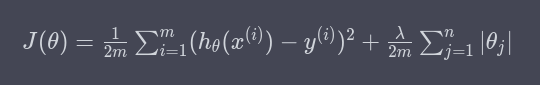
\includegraphics[width=1\linewidth]{pics/Formula_Ridge.png}
    \end{center}
    \caption{Formula of Ridge Regression}
    \label{fig:form_Ridge}
\end{figure}

Again, the model was evaluated against the test set. The results are as follows:
\begin{figure}[ht]
    \begin{center}
        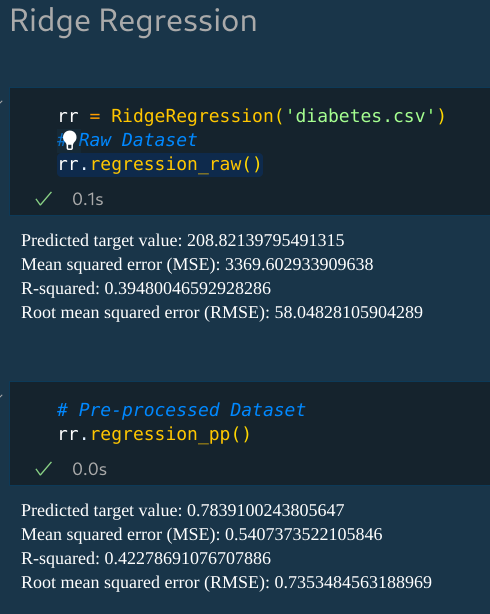
\includegraphics[width=1\linewidth]{pics/Result_Ridge.png}
    \end{center}
    \caption{Results of Ridge Regression}
    \label{fig:res_Ridge}
\end{figure}

\section{Part IV - Lasso Regression (Bonus)}
The Lasso Regression is also a regularized linear regression model. The formula is like this:
\begin{figure}[ht]
    \begin{center}
        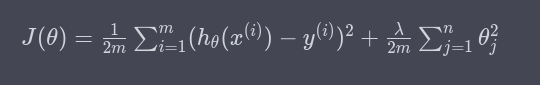
\includegraphics[width=1\linewidth]{pics/Formula_Lasso.png}
    \end{center}
    \caption{Formula of Lasso Regression}
    \label{fig:form_Lasso}
\end{figure}

Also, the resulting test perfomance was evaluated.
\begin{figure}[ht]
    \begin{center}
        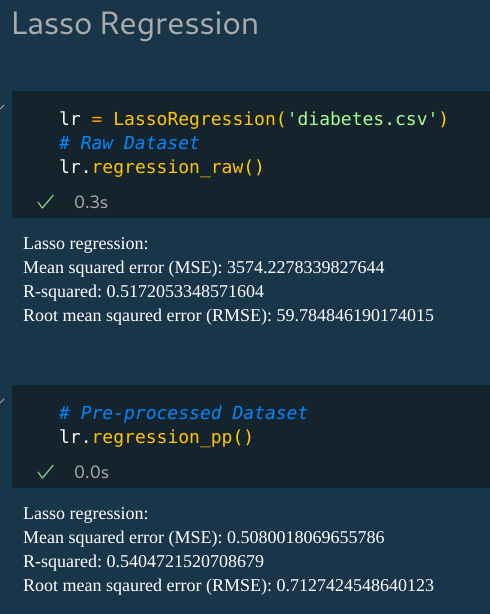
\includegraphics[width=1\linewidth]{pics/Result_Lasso.png}
    \end{center}
    \caption{Results of Lasso Regression}
    \label{fig:res_Lasso}
\end{figure}

\clearpage

\newpage
\onecolumn
\section*{APPENDIX}\label{sec:appendix}

This section houses the code.

\subsection*{Code for Part I}
\inputminted[%
breakanywhere=true,
breaklines,
mathescape,
linenos,
numbersep=5pt,
frame=single,
numbersep=5pt,
xleftmargin=0pt,
]{python3}{include/Predictor.py}

\subsection*{Code for Part II}
\inputminted[%
breakanywhere=true,
breaklines,
mathescape,
linenos,
numbersep=5pt,
frame=single,
numbersep=5pt,
xleftmargin=0pt,
]{python3}{include/LeastSquares.py}

\subsection*{Code for Part III}
\inputminted[%
breakanywhere=true,
breaklines,
mathescape,
linenos,
numbersep=5pt,
frame=single,
numbersep=5pt,
xleftmargin=0pt,
]{python3}{include/RidgeRegression.py}

\subsection*{Code for Part IV}
\inputminted[%
breakanywhere=true,
breaklines,
mathescape,
linenos,
numbersep=5pt,
frame=single,
numbersep=5pt,
xleftmargin=0pt,
]{python3}{include/LassoRegression.py}

\newpage

\thispagestyle{lastpage}
\end{document}